\documentclass[11pt,a4paper]{article}
\usepackage{ctex,amsmath,titlesec,amssymb,,graphicx,floatrow}
\usepackage[text={140mm,250mm},centering]{geometry}
\usepackage[margin=20mm]{geometry}
\begin{document}
\title{Hellinger-Reissner的动力分析}
\date{}
\maketitle
\section{薄板方程}
根据Kirchhoff板假设原理,在求解域$\Omega$内考虑厚度为$t$的薄板控制方程:
% \begin{displaymath}
    \begin{equation}
        \begin{split}
        \begin{cases}
        M_{\alpha\beta,\alpha\beta}+\bar q=\rho t a&\text {in} \; \Omega\\
        w=\bar w&\text{on}\;\Gamma_w\\
        \theta_n=w_{,n}=\bar \theta_n&\text{on}\;\Gamma_{\theta}\\
        V_n=Q_n+M_{ns,s}=\bar V_n&\text {on}\;\Gamma_V\\
        M_{nn}=\bar M_{nn}&\text {on}\; \Gamma_M\\
        w=\bar w&\text {at} \; c_w\\
        P=-[[M_{ns}]]\vert_{c_p}=\bar p&\text {at}\; c_P
        \end{cases}
        \end{split}
    \end{equation}
% \end{displaymath}
其中:
\begin{equation}
\begin{split}
    \begin{cases}
    w_{,n}=w_{,\alpha}n_{\alpha}\\
Q_n=n_{\alpha}M_{\alpha\beta,\beta}\\
M_{nn}=M_{\alpha\beta}n_{\alpha}n_{\beta},M_{ns}=M_{\alpha\beta n_{\alpha}s_{\beta}},M_{ns,s}=M_{\alpha\beta,\gamma}s_{\alpha}n_{\beta}s_{\gamma}
    \end{cases}
\end{split}
\end{equation}
其中,$M_{\alpha\beta}$为矩量$M$的弯曲和扭转分量,$\bar q$是施加的作用力,$\rho,t,a$分别表示板的密度,厚度,以及加速度。$\Gamma_w,\Gamma_{\theta},c_w$为强制边界边界条件以及相对应的挠度$\bar w$和转角$\bar \theta_n$,
$\Gamma_V,\Gamma_M,c_P$为自然边界条件,$V_n$表示的是等效剪切力,$M_{nn}$是法向弯矩,$P$是集中力,同时,所有的边界条件都满足如下关系式:
\begin{equation}
    \begin{split}
    \Gamma=\Gamma_w\cup\Gamma_V\cup\Gamma_{\theta}\cup\Gamma_M,c=c_w\cup c_P\\
    \Gamma_w\cap\Gamma_V=\Gamma_{\theta}\cap\Gamma_M=c_w\cap c_P=\varnothing
    \end{split}
    \end{equation}
并且$\pmb{n}=\{n_x,n_y\}^T,\pmb{s}=\{s_x,s_y\}$分别表示所在边界方向上的外法线方向和切线方向的分量\par
考虑具有线弹性各同向性材料的均匀板,其本构方程为:
\begin{equation}
    \begin{split}
    M_{\alpha\beta}=D_{\alpha\beta\gamma\eta}k_{\gamma\eta}=-D_{\alpha\beta\gamma\eta}w_{,\gamma\eta}
    \end{split}
    \end{equation}
其中
\begin{equation}
    \begin{split}
    D_{\alpha\beta\gamma\eta}=\bar D(\nu\delta_{\alpha\beta}\delta_{\gamma\eta}+\frac{1}{2}(1-\nu)(\delta_{\alpha\gamma}\delta_{\beta\eta}+\delta_{\alpha\gamma}\delta_{\beta\gamma}))
    \end{split}
    \end{equation}
并且,$k_{\alpha\beta}=-w_{,\alpha\beta}$为曲率张量$k$的分量,$\bar{D},E,\nu$分别为抗弯刚度,杨氏模量以及泊松比,和板的厚度$t$具有以下关系式:
\begin{equation}
    \begin{split}
    \bar D=\frac{Et^3}{12(1-\nu^2)}
    \end{split}
    \end{equation}
根据上述公式,$M_{nn},V_n,P$可以改写为:
\begin{equation}
    \begin{split}
    \begin{cases}
    M_{nn}=\mathcal{M}_{\alpha\beta}w_{,\alpha\beta}=-\bar D(\nu\delta_{\alpha\beta}+(1-\nu)n_{\alpha}n_{\beta})w_{,\alpha\beta}\\
    V_n=\mathcal{V}_{\alpha\beta}w_{,\alpha\beta}=-\bar D(\frac{\partial}{\partial x_{\alpha}}n_{\beta}+(1-\nu)\frac{\partial}{\partial x_{\gamma}}s_{\alpha}n_{\beta}s_{\gamma})w_{,\alpha\beta}\\
    P=\mathcal{P}_{\alpha\beta}w_{,\alpha\beta}=-(\bar D(1-\nu)n_{\alpha}s_{\beta})w_{,\alpha\beta}
    \end{cases}
    \end{split}
    \end{equation}





\section{数值算例}
\subsection{一维简支梁问题}
考虑如图1所示的一维简支梁问题,简支梁在跨中受到谐波点力$F(t)=F_0sin(wt)$,其中$\omega=\pi,F_0=10$。简支梁的几何和材料性质为:长度$L=10$,截面宽度$b=1$,厚度$t=1$,密度$\rho=2500$,一维简支梁的杨氏模量为$E=2\times10^6$。该问题的解析解为:
\begin{equation}
\begin{split}
    w(x,t) = \frac{{2{F_0}}}{{\rho AL}}\sum\limits_{i = 1,3,5...}^\infty  {(\sin (\frac{{i\pi }}{2})\frac{{\sin (i\pi x/L)}}{{{\omega ^2}_i - {\omega ^2}}} \times (\sin (\omega t) - \frac{\omega }{{{\omega _i}}}\sin ({\omega _i}t)))} \\ 
\end{split}
\end{equation}
其中
\begin{equation}
{\omega _i} = \frac{{{i^2}{\pi ^2}}}{{{L^2}}}\sqrt {\frac{{EI}}{{\rho A}}} 
\end{equation}
其中,$A=b\times h$表示为简支梁横截面的面积。\par
\begin{figure}[!h]
\centering
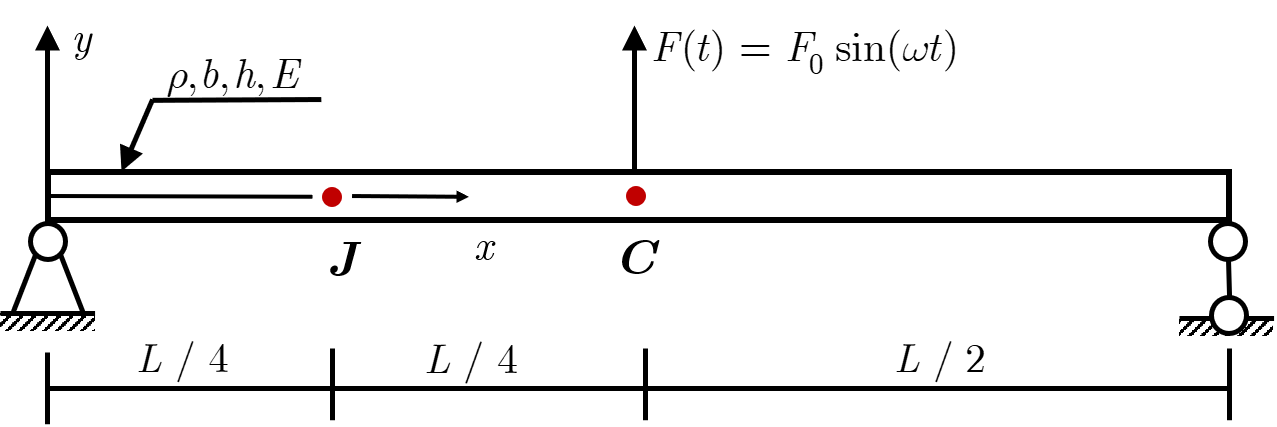
\includegraphics[scale=0.5]{firgure/beam.png}
\caption{一维简支梁问题模型}
\end{figure}
\begin{figure}[!h]
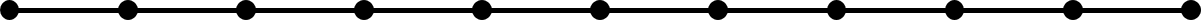
\includegraphics[scale=0.5]{firgure/beam.mesh.png}
\caption{一维简支梁问题模型节点离散}
\end{figure}
一维简支梁的求解域以图2所示采用11个均匀间隔的节点进行离散分析,算例采用具有三次和四次基函数的无网格近似函数计算,核函数的相对影响域分别为3.5\\和4.5。时间设置步长为$triangle t=0.01s$。
为了方便起见,定义挠度误差$error=\omega^h(x,t)-\omega^{\varepsilon}(x,t)$来定义各种方法的准确性,图和图分别表示的是一维简支梁模型采用三次和四次基函数中心点C的挠度时间历程和挠度误差,
从图3和图4可以清楚的看出采用RKGSI-HR方法的解精度最好,挠度误差几乎为0,而采用GI-2和GI-5方法的误差几乎相同,相较于RKGSI-HR方法的误差较大,充分说明了RKGSI-HR方法在频率计算方法的精确性。
\subsection{简支方板问题}
如图5所示,二维简支方板在板心处受到正弦集中力的作用,其中几何和材料参数为:长度为$a=10$,厚度$t=0.05$,密度$\rho=2\times 10^{11}$,泊松比$\nu=0.3$,集中力$F_0=1000$,频率$\theta=\pi$,
简支方板的精确解为:
\begin{equation}
\begin{split}
    w (x,y,t) = \mathop \sum \limits_{m = 1}^\infty  \mathop \sum \limits_{n = 1}^\infty  {W_m}_n(x,y){\eta _m}_n(t) 
\end{split}
\end{equation}
其中
\begin{equation}
\begin{split}
&{W_m}_n(x,y) = \frac{2}{{a\sqrt {\rho t} }}\sin (\frac{{m\pi x}}{a})\sin (\frac{{n\pi y}}{a})\\
&{\eta _m}_n(t) = \frac{{2{F_0}}}{{({\omega ^2}{{_m}_n} - {\theta ^2})a\sqrt {\rho t} }}\sin (\frac{{m\pi }}{2})\sin (\frac{{n\pi }}{2}) \times (\sin \theta t - \frac{\theta }{{{\omega _m}_n}}\sin {\omega _m}_nt)
\end{split}
\end{equation}
\begin{figure}[!h]
\begin{floatrow}
\ffigbox{\caption{简支方板问题模型}}{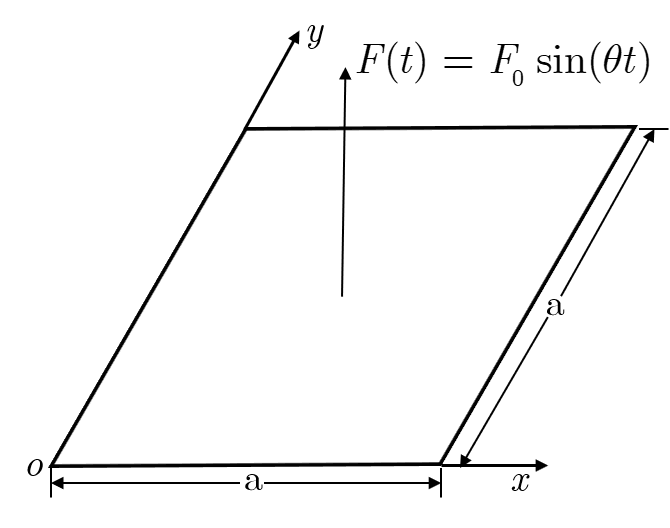
\includegraphics[scale=0.65]{firgure/plate.png}}
\ffigbox{\caption{简支方板问题离散}}{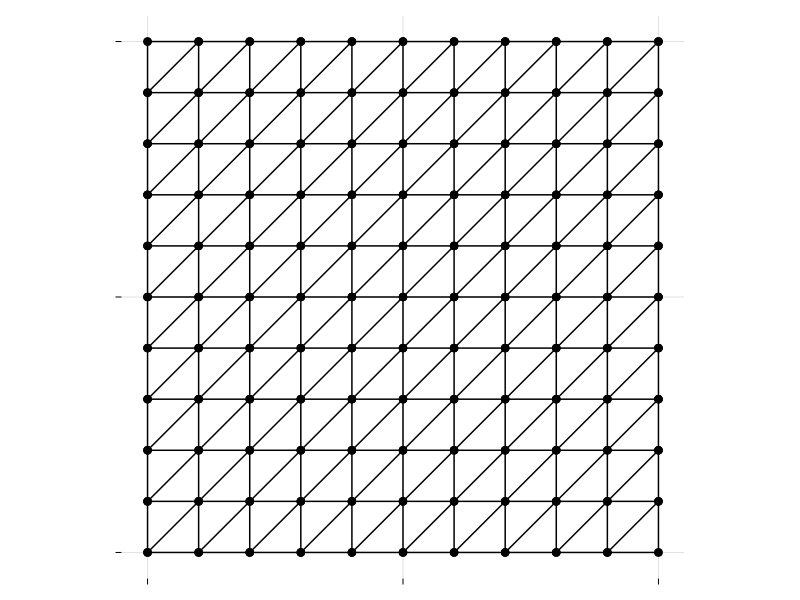
\includegraphics[scale=0.3]{firgure/plate.mesh.png}}
\end{floatrow}
\end{figure}
简支方板的求解域根据图4所示的采用$11\times 11$的均匀间隔点进行离散分析,算例采用具有三次和四次基函数的无网格近似计算,核函数相对应的影响域分别为3.5\\和4.5.时间设置步长为$\triangle t=0.01s$。
图和图分别表示的是简支方板用三次和四次基函数时的中心点挠度的时间历程和挠度误差,结果表明在二维情况下采用RKGSI-HR的方法中心挠度误差几乎为0,同时也小于采用高斯积分GI-2和GI-5所得出的挠度误差,
进一步说明了RKGSI-HR方法在计算高阶薄板问题频率计算方面的准确性。


\end{document}